% !TeX root = ../main.tex
% Add the above to each chapter to make compiling the PDF easier in some editors.

\chapter{Implementation}\label{chapter:implementation}
Chapter Introduction


\section{Concept: Features and Interaction Capabilities of the App}
In this section, we explore the expected features and capabilities crucial for our objectives and the necessary interaction capabilities from an end user's perspective.\\
We start with the visualisation capabilities of the benchmark data, where the goal is to easily identify performance bottlenecks. This involves pinpointing interesting queries with distinct performances for subsequent in-depth analysis.\\
For deeper analysing and achieving a profound understanding of diverse performance results within queries, the application should support a focus on individual queries. Users should be able to view the performance of a single query from various perspectives, providing a comprehensive image. Comparative analysis across queries from different database systems or even the same database but with different configurations is also essential.\\ 
Then, we examine the requirements for a suitable dashboard that contains the main part of the performance visualisations. Multiple views are necessary to construct a complete understanding of the current point of interest. The optimal structure of these views may vary depending on the point of interest. The flexibility of a drag-and-drop solution for structuring views allows users to tailor the overview according to their specific interests.\\
Finally, we examine the capability of the system to facilitate collaboration and knowledge sharing. The application should enable the saving and sharing of potential findings. This involves saving the interface configuration of the analysis for sharing with other users. Recipients should be able to upload the received configuration, gaining access to the same data and visualisation structure for collaborative exploration.


\subsection{Visualising Benchmark Data}
Visualising Benchmark Data includes multiple aspects. It involves the import of the actual data, where a proper way of importing the data should be provided. We also cover the utilized plots and charts for the data visualization. In addition to visualisation, we offer a comprehensive table view of the data.


\subsubsection{Import of Performance Data}

The first step working with the Benchy Viewer is to import a file containing the performance data which should be visualised. The file needs to follow the format introduced in Section \ref{sec:input-file-structure}. Figure~\ref{fig:input-process-flow} summarizes the import of the input file in a process diagram.

\begin{figure}[h]
  \centering
  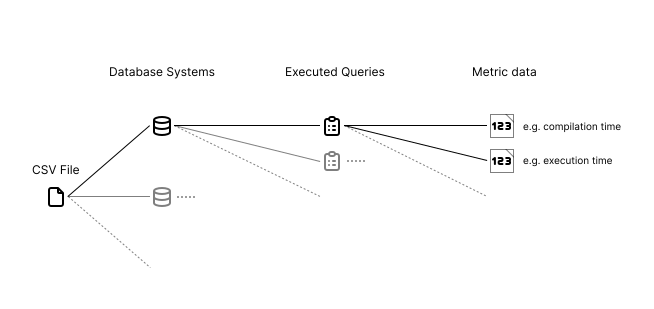
\includegraphics[width=1\linewidth]{figures/csv-structure.pdf}
  \caption{Import process of input data}
  \label{fig:input-process-flow}
\end{figure}

Chart beschreiben.


\subsubsection{Charts and Plots}

We aim to offer a dashboard containing multiple data views. To prevent UI clutter, a universal legend of database system instances is suitable, eliminating the necessity to display a legend in every chart. In the legend depicted in Figure~\ref{fig:legend} all database systems included in the benchmark data are presented as coloured toggles, allowing users to activate or deactivate their appearance in the visualisation.

\begin{figure}[h]
    \centering
    \includegraphics[width=1\linewidth]{figures/legend.png}
    \caption{Gobal legend of all database systems contained in the imported performance data.}
    \label{fig:legend}
  \end{figure}

The preceding visualization solution \textcolor{red}{Referenz auf PDF} shows essential benchmark visualisations, offering both a comprehensive overview of all queries and a detailed examination of each individual query.\\
It commences with a comparative analysis of each query using a bar chart. Similar to Figure~\ref{fig:bar-chart}, this chart displays queries from various database systems on the X-Axis, with the total time presented on the Y-Axis. 

\begin{figure}[h]
    \centering
    \includegraphics[width=1\linewidth]{figures/bsp-bar.png}
    \caption{Bar chart visualises the totals time in ms of different queries.}
    \label{fig:bar-chart}
  \end{figure}

Bar plots stand out as a versatile visualization method, particularly when tasked with presenting the performance metrics of multiple queries. Their inherent clarity, with the length of each bar directly corresponding to a specific performance metric such as compilation time or execution time, makes them well-suited for diverse scenarios.\\
The straightforward visual comparison they offer is a notable strength. With each query distinctly represented by a separate bar, variations in performance become immediately apparent.\\
This quality proves especially valuable for our objective of identifying outliers, as these exceptional values are easily noticeable.

To facilitate a quick and clear overview of all queries, violin charts are employed. These charts not only provide an initial glimpse of the overall system performance but also offer distribution insights, including the shape and density of the data. They can also be combined with box plots to get a concise summary of the distribution of the results, displaying key statistics such as the median and quartiles.

\begin{figure}[h]
    \centering
    \includegraphics[width=1\linewidth]{figures/bsp-violin-boxplot-points.png}
    \caption{Violin charts visualise the totals time in ms of different queries. The left variant contains a box plot and the right variant contains all data points.}
    \label{fig:violin-chart}
  \end{figure}

Within the Benchy Viewer violin plots that contain data points, as shown in Figure~\ref{fig:violin-chart} on the right side, additionally allow you to hover over a data point. This action highlights the corresponding query in the violins of the other database systems. We will explore this hover feature further in \ref{sec:hover-feature}.

In the context of providing a clear and comparative understanding of how different systems perform relative to a chosen baseline, the metrics maximum slowdown and maximum speedup become crucial. They offer a comprehensive view of the range of performance variations. Maximum slowdown indicates the worst-case scenario of reduced performance, while maximum speedup highlights the most significant improvement achieved.

\textbf{Slowdown} indicates how much slower a specific system is compared to the baseline system. It is calculated as the ratio of the time taken by the system under consideration to the time taken by the baseline system. A slowdown value greater than 1 implies that the system is slower than the baseline. For example, a slowdown of 1.5 means the system is 1.5 times slower than the baseline.\\
Identifying slowdowns is crucial for pinpointing areas of inefficiency or performance bottlenecks in a system. It helps in understanding where improvements are needed.

\textbf{Speedup}, on the other hand, quantifies how much faster a specific system is compared to the baseline system. It is calculated similarly to slowdown but in the reverse manner. A speedup value greater than 1 implies that the system is faster than the baseline. For example, a speedup of 2 means the system is twice as fast as the baseline.\\
Knowing the speedup is essential to highlight improvements. It indicates the effectiveness of optimizations or enhancements made to the system compared to the baseline.

The Benchy Viewer employs tables to showcase the maximum slowdown and maximum speedup, visualized in Figure~\ref{fig:slowdown-speedup-chart}, where the maximum slowdown is displayed on the left side and the maximum speedup on the right side using Umbra as the baseline system. The use of cell colors in the table serves as an effective visual indicator of performance outliers. Intensity in color corresponds to the extent of the outlier, offering a rapid understanding of the range and distribution between these extreme values. This color-coded representation aids users in identifying and assessing the significance of performance variations across different systems.

\begin{figure}[h]
  \centering
  \includegraphics[width=1\linewidth]{figures/bsp-table-speedup-slowdown.png}
  \caption{Tables showcase the maximum slowdown and the maximum speedup using color intensity to indicate performance outliers.}
  \label{fig:slowdown-speedup-chart}
\end{figure}

The tables are organized based on the resulting ratio.\\
 In the maximum slowdown tables, the arrangement is ascending, placing the slowest queries of the baseline system compared to the faster alternative system at the top.\\
 Conversely, in maximum speedup tables, the sorting is descending, presenting the fastest queries of the baseline system compared to the alternative system at the forefront. This sorting strategy provides a logical structure to quickly identify and compare performance differences in either scenario.

Scatter plot is also used for displaying the speedup and slowdown

\subsubsection{Hover Feature}\label{sec:hover-feature}

\subsubsection{Data Viewer}


\subsection{Deeper Inspection and Comparison of selected Queries}
Query Plan
DBs aktivieren/ deaktivieren
\subsection{Flexible Interface Hub}
\subsubsection{Drag and Drop}
DnD Sektionen und Dnd Charts
\subsubsection{Chart Configurations}
- Metrics auswählen
- tabele und scatter: speed-up/ slow-down
- Scale: Linear/ Log/ Throuput
- Violin: scatter und boxplot
\subsection{Saving and Sharing the Application State}


\section{Design}
\subsection{User Interface}
\subsection{Page Structure and Navigation}
\subsubsection{}

\section{Data Structure}
\subsection{Overall Project Structure}
\subsection{Input File and Benchmark Data}
\subsection{Plot Options}
\subsection{Visualisation Arrangement Data Structure}
\subsection{Query Plan}
\subsubsection{Visualisation Parameters}
\subsubsection{Query Plan Data Structure}

\section{Integration of Plotly-React for Data Visualization}
\subsection{Types of Plots and Charts}
\subsection{Hover Feature}
\subsection{Selected Query Feature}

\section{Integration of semantic-diff-tool}
\subsection{Business Logic}
\subsection{Settings}
\subsection{UI}